\documentclass{cmn}
\usetikzlibrary{shapes.geometric}

\def\scopeXSep{32.5mm}
\def\triangleYShift{5.4mm}
\def\triangleXShift{1.1mm}

\tikzset{
  tree/.style={
    level distance=10mm,
    level 1/.style={sibling distance=14mm},
  },
  circleNode/.style={draw,circle,inner sep=1.75mm},
  triangle/.style={
    draw,
    isosceles triangle,
    isosceles triangle apex angle=60,
    shape border rotate=90,
    minimum height=10mm
  },
  triangleLeftNode/.style={
    triangle,
    xshift=\triangleXShift,
    yshift=-\triangleYShift
  },
  triangleRightNode/.style={
    triangle,
    xshift=-\triangleXShift,
    yshift=-\triangleYShift
  }
}

\begin{document}
  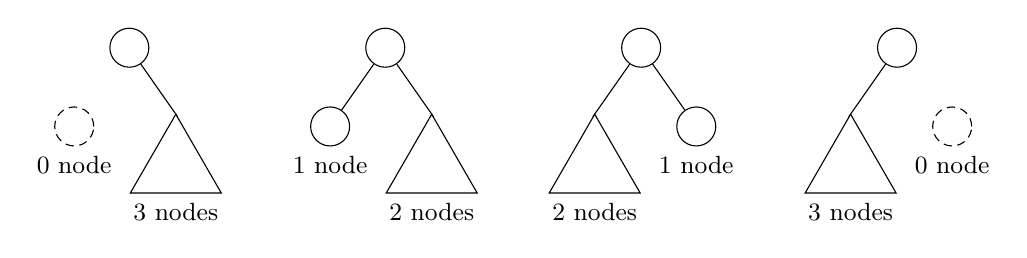
\begin{tikzpicture}
    \begin{scope}[tree]
      \node[circleNode] {}
        child {node[circleNode,densely dashed,label=below:{\small 0 node}] {} edge from parent[draw=none]}
        child {node[draw=none] {}
          {node[triangleRightNode,label=below:{\small 3 nodes}] {}}
        };
    \end{scope}

    \begin{scope}[tree,xshift=\scopeXSep]
      \node[circleNode] {}
        child {node[circleNode,label=below:{\small 1 node}] {}}
        child {node[draw=none] {}
          {node[triangleRightNode,label=below:{\small 2 nodes}] {}}
        };
    \end{scope}

    \begin{scope}[tree,xshift=2*\scopeXSep]
      \node[circleNode] {}
        child {node[draw=none] {}
          {node[triangleLeftNode,label=below:{\small 2 nodes}] {}}
        }
        child {node[circleNode,label=below:{\small 1 node}] {}};
    \end{scope}

    \begin{scope}[tree,xshift=3*\scopeXSep]
      \node[circleNode] {}
        child {node[draw=none] {}
          {node[triangleLeftNode,label=below:{\small 3 nodes}] {}}
        }
        child {node[circleNode,densely dashed,label=below:{\small 0 node}] {} edge from parent[draw=none]};
    \end{scope}
  \end{tikzpicture}
\end{document}
